\documentclass[a6paper, 11pt, parskip=half, DIV=15]{scrartcl}

\usepackage[dvipsnames]{xcolor}
\usepackage{tikz}

\usepackage{ragged2e}
% Minimize unwanted hyphenation
\tolerance=1
\emergencystretch=\maxdimen
\hyphenpenalty=1
\hbadness=10000

\usepackage{booktabs}
\usepackage{caption}
\captionsetup{justification=raggedright,
              singlelinecheck=false}

\usepackage{fontspec}
\setmainfont{Tex Gyre Schola}
%\setmainfont{Qwigley}

\usepackage{eso-pic}
\usepackage{contour}
\contourlength{0.25mm}
\contournumber{1024}

\definecolor{SunriseBlue}{HTML}{A1A6CF}
%\definecolor{SunriseBlue}{HTML}{A9C2E5}
\setkomafont{section}{\setmainfont{Fredoka-Bold}\LARGE\color{SunriseBlue}}
\setkomafont{subsection}{\setmainfont{Fredoka-Bold}\Large\color{SunriseBlue}}
\setkomafont{subsubsection}{\setmainfont{Fredoka-Bold}\large\color{SunriseBlue}}

% Adjust spacing before and after section headings
\RedeclareSectionCommand[
  runin=false,
  beforeskip=1.0\baselineskip,
  afterskip=-0.0\baselineskip
]{section}

% Adjust spacing before and after subsection headings
\RedeclareSectionCommand[
  runin=false,
  beforeskip=1.0\baselineskip,
  afterskip=-0.0\baselineskip
]{subsection}

% Adjust spacing before and after subsubsection headings
\RedeclareSectionCommand[
  runin=false,
  beforeskip=1.0\baselineskip,
  afterskip=-0.0\baselineskip
]{subsubsection}


\usepackage{enumitem}
\setlist[description]{labelindent=0pt, labelsep=\widthof{ }, leftmargin=\widthof{\textbf{License: }}, font=\setmainfont{Tex Gyre Schola}\bfseries}

\usepackage[hang,flushmargin]{footmisc}
\newcommand\blfootnote[1]{%
  \begingroup
  \renewcommand\thefootnote{}\footnote{#1}%
  \addtocounter{footnote}{-1}%
  \endgroup
}

\renewcommand{\thefootnote}{\fnsymbol{footnote}}
\renewcommand{\footnoterule}{%
  \kern -3pt
  \hrule width \textwidth height 0.5pt
  \kern 2pt
}

\usepackage[hidelinks]{hyperref}
\usepackage[type={CC}, version={4.0}, modifier={by-nc-nd}]{doclicense} % Add text and icons for creative commons license
%\usepackage{array}

\raggedright
\pagestyle{empty}
%\pagecolor{SkyBlue!50}
\begin{document}

\begin{titlepage}
\AddToShipoutPictureBG{
\begin{tikzpicture}[remember picture, overlay]
%	\node () at (current page.center) {\includegraphics[width=\pagewidth, height=\pageheight]{Images/aloft_cover_background.png}};
	\node () at (current page.center) {\includegraphics[width=\pagewidth, height=\pageheight]{Images/aloft_front_cover_background.png}};
\end{tikzpicture}
}

\enlargethispage{3.0\baselineskip}
\Huge
\vspace*{-1.0\baselineskip}
{
\setmainfont[Scale=2.2375]{Oi}
\begin{center}
\textcolor{white}{Aloft}
\end{center}
}
\vfill
\huge
\setmainfont[Scale=1.05]{Playball}
\begin{center}
\textcolor{white}{Designed by Michael Purcell}
\end{center}
\end{titlepage}


\ClearShipoutPicture
\enlargethispage{1.75\baselineskip}
\section*{Overview}
Aloft is a game for two to five players. It can be played in about thirty minutes and is intended for players who are at least eight years old.

During the game, you will launch a flight of hot-air balloons. You will try to ensure that your balloons end up in the best positions in the resulting formation.

\section*{Components}
\begin{itemize}[nosep]
  \item 47 sky tiles
  \item 3 launch-site tiles
  \item 15 balloon pieces
  \item 6 color cards
  \item 30 launch tokens
  \item 18 scoring tokens
  \item 4 cloud tokens
\end{itemize}

\newpage
\enlargethispage{1.75\baselineskip}
\section*{Set Up}
\begin{enumerate}

  \item In a two or three-player game, give each player two secret color cards. Otherwise, give each player one secret color card.
%  Do not reveal your color card(s) to the other players.
 
  \item Build the game board by laying out forty-six sky tiles in four rows: ten in row one, eleven in row two, twelve in row three, thirteen in row four.
  
  Each row should be centered and offset from any rows adjacent to it by half the width of one sky tile.
  
  \item Give the last sky tile to the first player.
  
  \item Place the three launch-site tiles below the game board as shown in the set up diagram below.
  
  \item Place a cloud token on the left-most sky tile in each row.

  \item Sort the launch tokens by color and place them to one side of the game board.

  \item Place the balloon pieces at the bottom of the game board. 

\end{enumerate}

\newpage
\enlargethispage{1.75\baselineskip}

\subsection*{Set Up Diagram}

\begin{center}
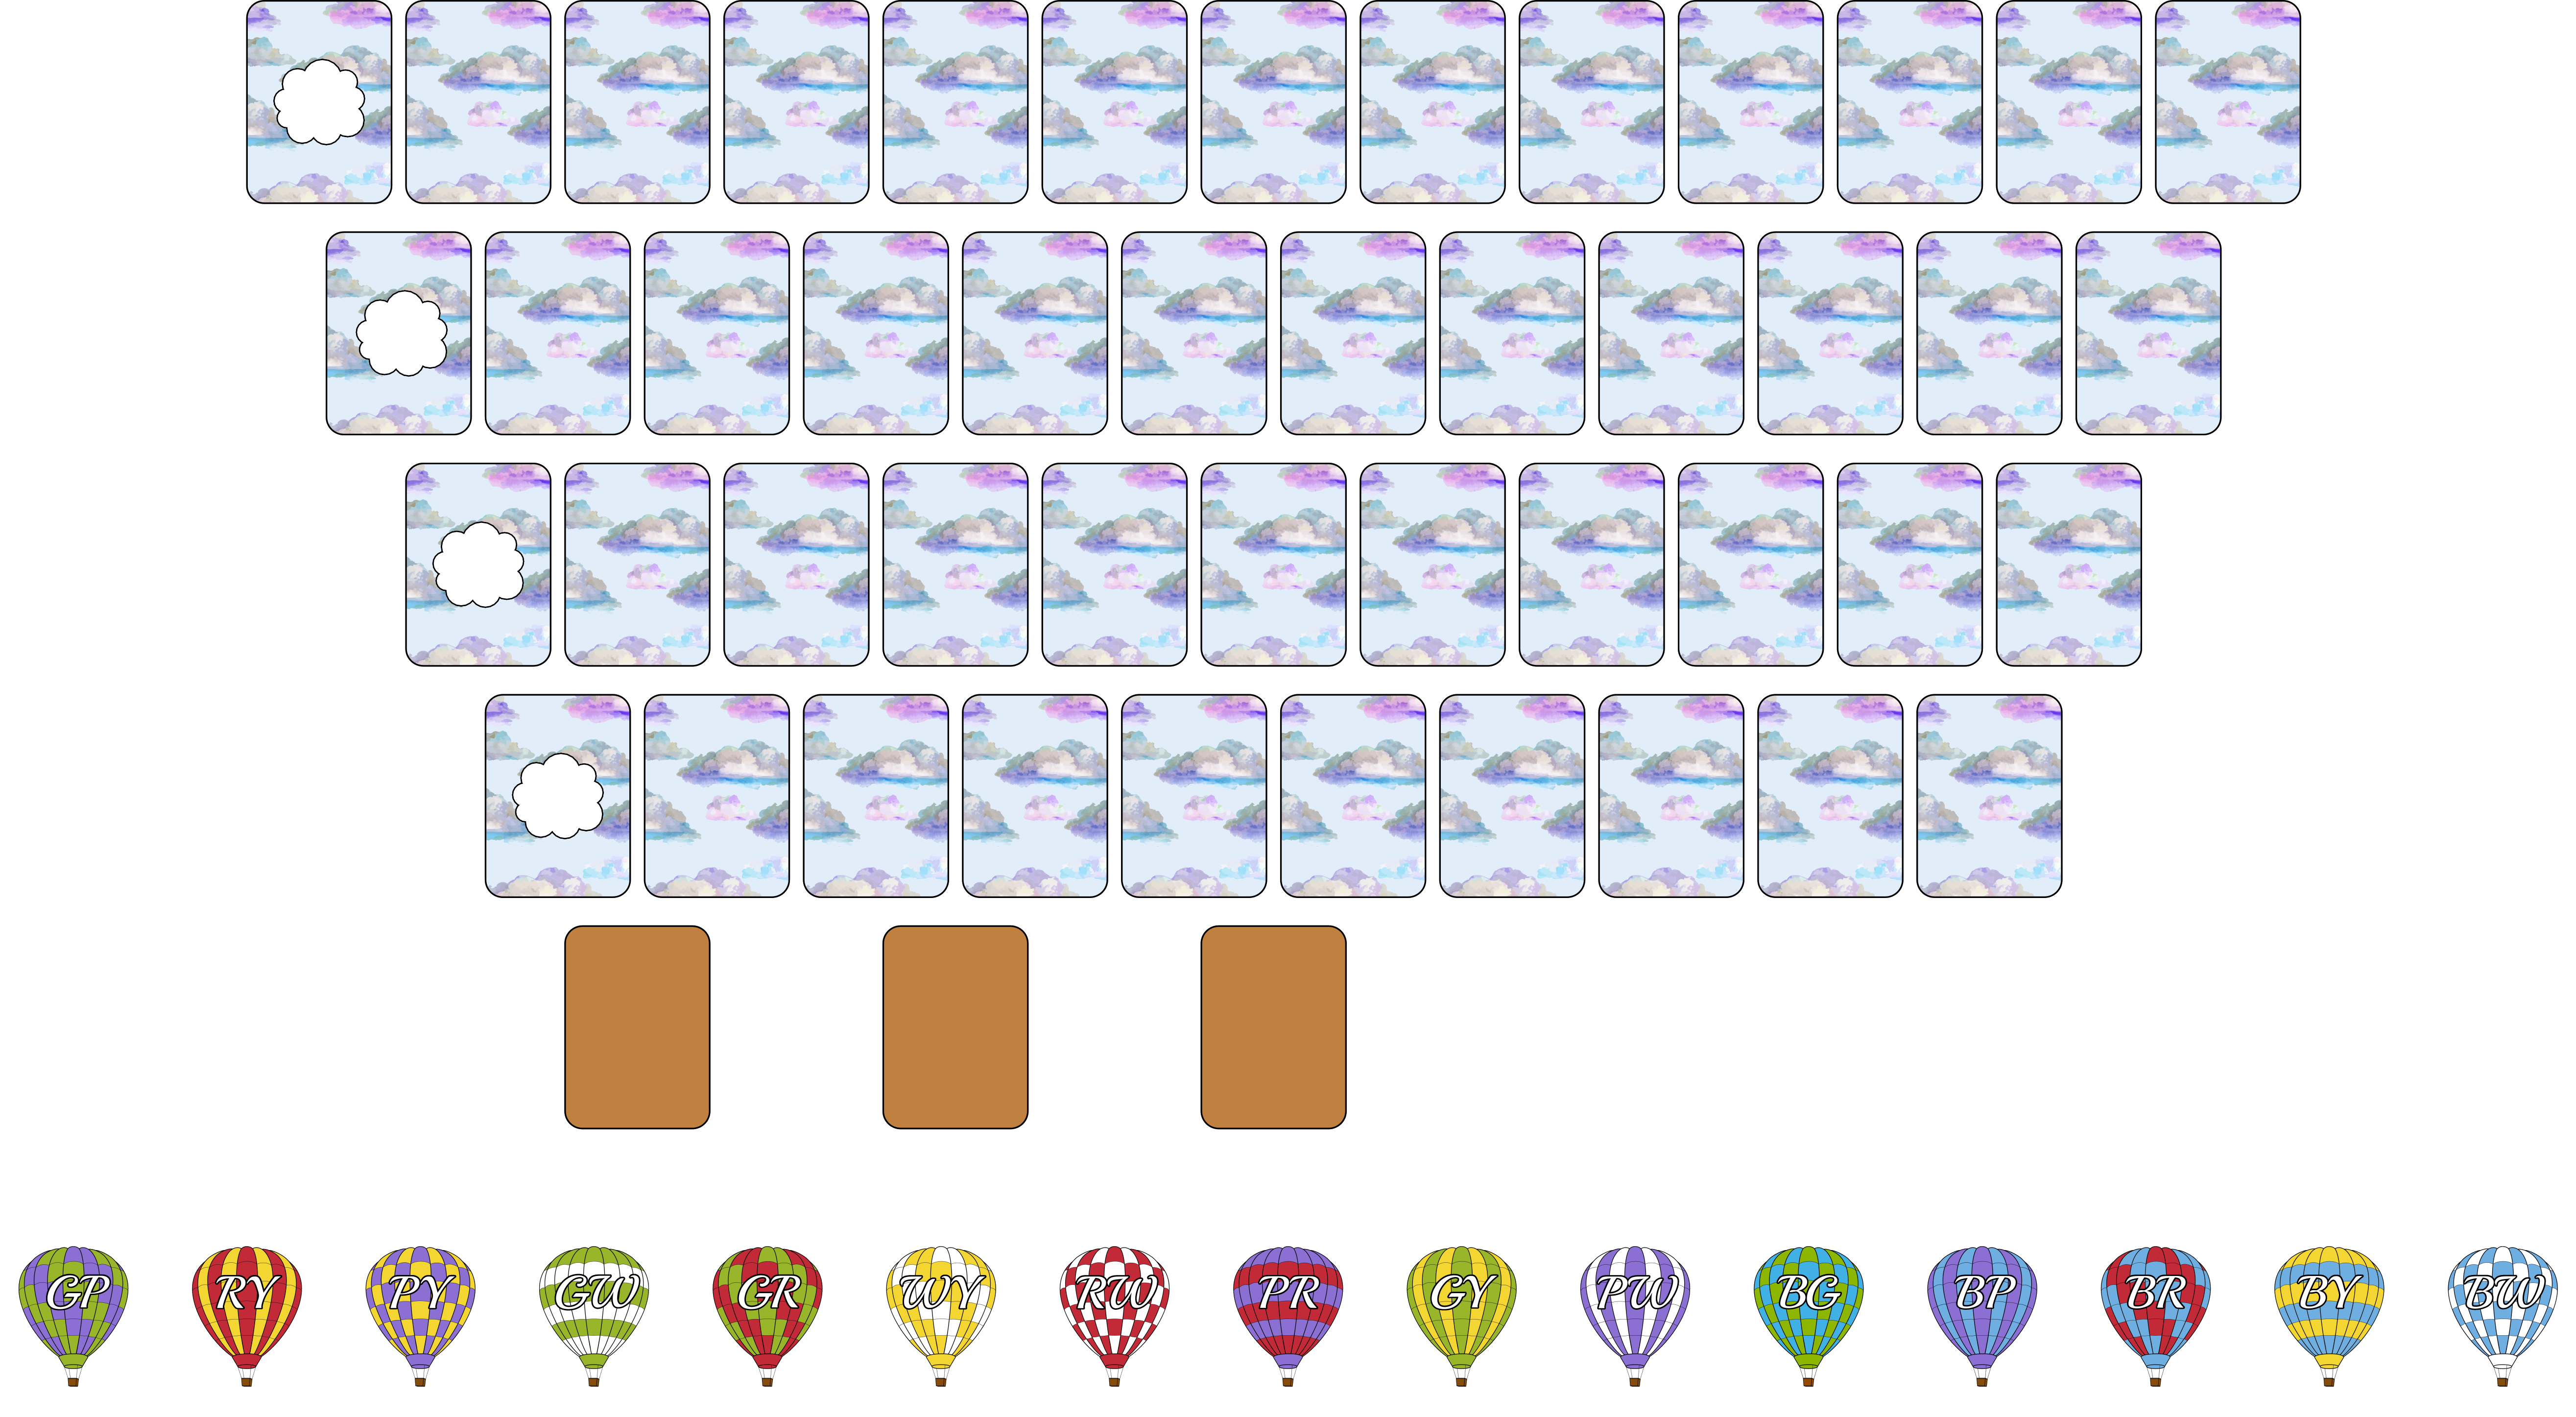
\includegraphics[width=\textwidth]{Images/set_up_diagram2.png}
\end{center}


\section*{Gameplay}
On your turn, you will both:
\begin{enumerate}[nosep]
  \item Advance a balloon.
  \item Blow the wind.
\end{enumerate}

The game ends immediately when any sky tile with a cloud token on it is pushed off of the game board (see {\setmainfont{Fredoka-Bold}\textcolor{SunriseBlue}{Blow the Wind}}).


\newpage
\enlargethispage{1.75\baselineskip}

\subsection*{Advance a Balloon}
%Each balloon will advance through a series of states: packed, inflated, and flying.
All balloons start in the packed state.

\begin{description}[leftmargin=0pt]
  \item[Inflate:] To inflate a balloon that is packed, place it on top of an unoccupied launch-site tile.
  
    When you inflate a balloon, collect one launch token for each color on that balloon. Put one of these launch tokens on the balloon piece. Put the other in your personal \emph{collection}.

  \item[Launch:] To launch a balloon that has been inflated, move it to one of the two sky tiles directly above its launch-site tile. 
  
  When you launch a balloon, collect the launch token thereon and add it to to your collection.
  
  \item[Ascend:] To advance a balloon that is flying, move it to one of the two sky tiles directly above its current location.
  \begin{itemize}
    \item Balloons that are flying may never be horizontally adjacent to one another.
    \item Balloons may not move off the top edge of the board.
    \item Balloons may not move onto sky tiles that have cloud tokens on them.
  \end{itemize}
\end{description}

\newpage
\enlargethispage{1.75\baselineskip}

\subsubsection*{Double Moves}
When you advance a balloon, you may optionally spend a launch token from your collection to make a \emph{double move}.

To do so, first choose a launch token to spend. The launch token that you spend must not match either of the colors on the balloon that you are advancing. Place the launch token that you spend back in the supply.

Then, advance a single balloon two times. You may not take an inflate action as part of a double move. That is, when you make a double move with a balloon it must already either be inflated or flying.

When you make a double move with a balloon, you may move that balloon through sky tiles that would otherwise be inaccessible, either due to adjacency rules or the presence of cloud tokens. The balloon that you move must be in a legal position at the end of your turn.



\newpage
\enlargethispage{1.75\baselineskip}

\subsection*{Blow the Wind}
To blow the wind, you will use the extra sky tile to push the tiles that comprise one row of the game board one position to the right.

Every sky tile has a number on its back. This number indicates the row where that tile will be inserted.

You will always push the extra tile into the left-hand side of the game board.
Doing so will cause all of the other tiles in that row, and any balloon pieces that are on those tiles, to slide one position to the right.

After you insert a sky tile in a row, remove the rightmost sky tile from that row.
If the tile you remove has a balloon piece on it, remove that balloon piece from the game.
If the tile you remove has a cloud token on it, the game ends immediately.

Hand the sky tile that you removed to the next player.
They will use this tile to blow the wind at the end of their turn.


\newpage
\enlargethispage{1.75\baselineskip}
\section*{Scoring}

There are two ways to score, achievement scoring and formation scoring. The player with the highest combined score wins the game.

\subsection*{Achievement Scoring}
Your achievement score is determined by the launch tokens that you collected.

\begin{enumerate}
	\item Sort your launch tokens by type. Sort your launch tokens by color.
	\item Score 10 points for each \emph{rainbow set} consisting of one token of each color.
	\item Score points based on the size of each set of launch tokens in your collection according to the following table.
\end{enumerate}
	\begin{center}
	\begin{tabular}{lcccccc}\toprule
	Set Size & 0 & 1 & 2 & 3 & 4 & 5 \\\midrule
	Points & 0 & 1 & 3 & 6 & 10 & 15\phantom{0} \\\bottomrule
	\end{tabular}
	\end{center}


\newpage
\enlargethispage{1.75\baselineskip}

\subsection*{Formation Scoring}
Use the scoring tokens to indicate the number of points scored by each balloon.
\begin{enumerate}
  \item Place the scoring token numbered ``1'' on the leftmost balloon in the bottom row of the final formation.
  \item Scanning from left to right and bottom to top, place scoring tokens on the other balloons in the formation, placing the token with lowest remaining number on each balloon as you encounter it.
\end{enumerate}

Your formation score is the sum of the scores for balloons on which your color(s) appear.

\vfill

\begin{figure}[hb]
\centering
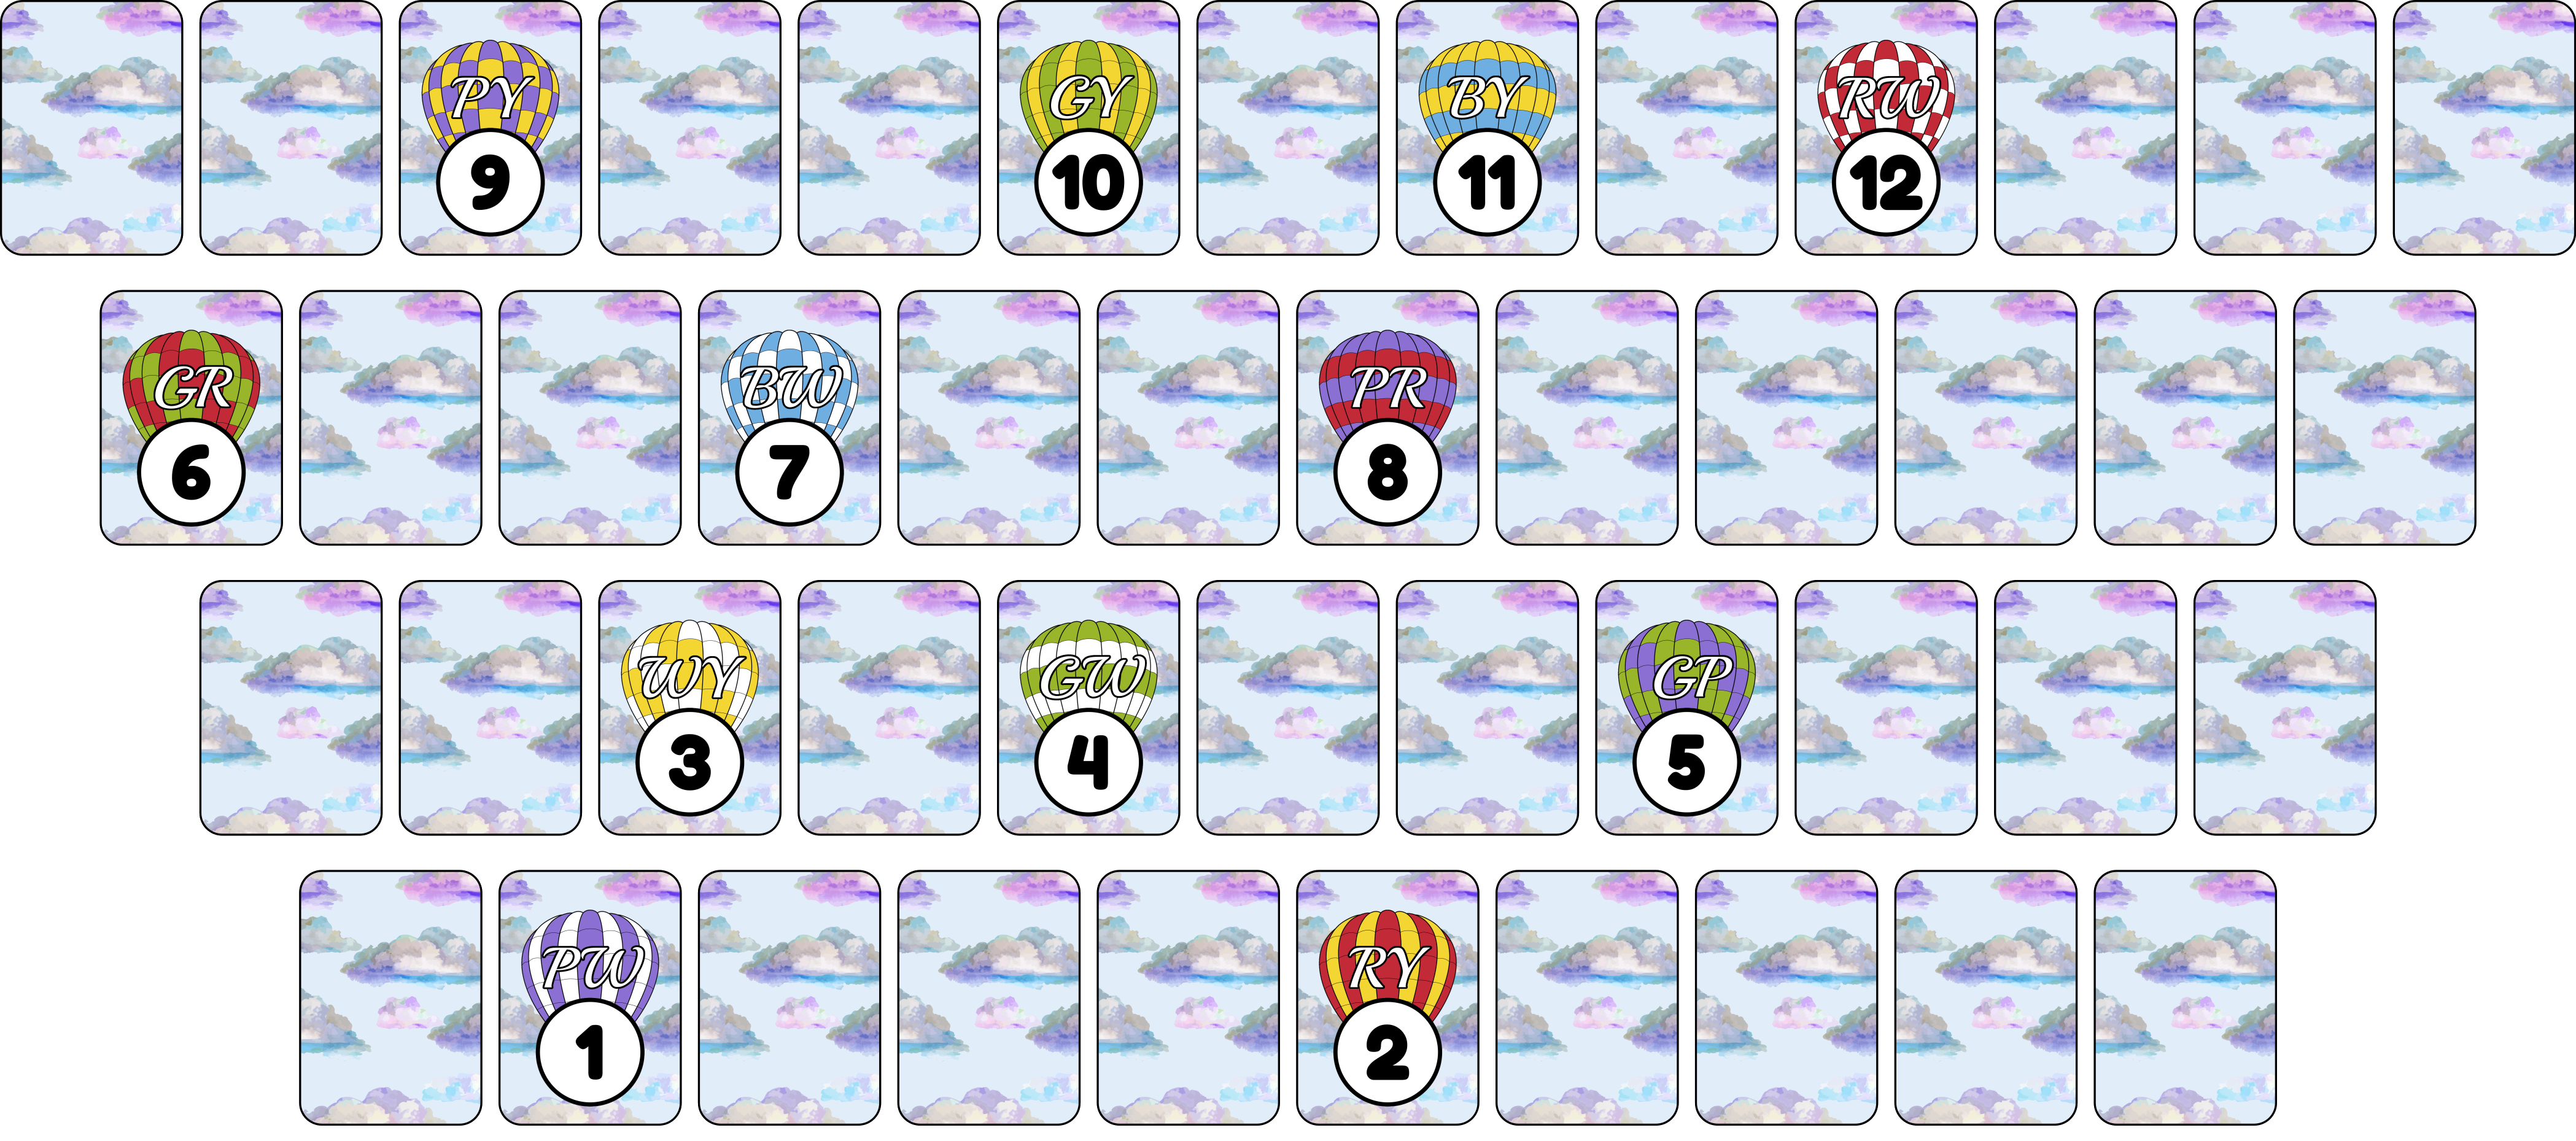
\includegraphics[width=0.8\textwidth]{Images/scoring_diagram2.png}
\caption*{\textbf{Example:} The red player's formation score\\is 28: 12 points for {\setmainfont{Playball}RW}, 8 points for {\setmainfont{Playball}PR},\\6 points for {\setmainfont{Playball}GR}, and 2 points for {\setmainfont{Playball}RY}.}
\end{figure}

 \newpage
 \AddToShipoutPictureBG{
\begin{tikzpicture}[remember picture, overlay]
%	\node () at (current page.center) {\includegraphics[width=\pagewidth, height=\pageheight]{Images/aloft_cover_background.png}};
	\node () at (current page.center) {\includegraphics[width=\pagewidth, height=\pageheight]{Images/aloft_back_cover_background.png}};
\end{tikzpicture}
}
\phantom{Aloft}
\end{document}